%! Tex Root = ../proposal.tex

\begin{frame}{Personal Research}

Mention my previous research

Show how it supports and solves some of the issues mentioned in the challenges

Quick summary of previous research
\end{frame}

\begin{frame}{Proposed Approach} % -----------------------------------%
  \begin{itemize}
      \item \Emph{Reachability set} on \Poincare section allows for systematic transfer design
        \begin{itemize}
            \item Transfer design on lower dimensional subspace
            \item Simple method to incorporate effects of low-thrust 
            \item Avoids the issue of determining initial conditions
        \end{itemize}
        \pause
      \item Extension of previous work in planar three-body problem     
  \end{itemize}

  \note[itemize]{
    \item Reachability set avoids the need to pick initial conditions
    \item We compute on a lower dimensional surface
  }
\end{frame} %--------------------------------------%

\begin{frame}{\Poincare map}
\begin{itemize}
    \item Intersection of a periodic orbit with a lower dimensional subspace, called the \Poincare section
    \pause
        \begin{itemize}
            \item Can be considered a discrete map 
        \end{itemize}
        \pause
    \item Useful for investigating the stability and structure 
    \pause
    \item Define a \Poincare section \( \Sigma \) 
        \begin{itemize}
            \item Used for initial and target periodic orbits
            \item Subspace for the \Emph{reachability set}
        \end{itemize}
\end{itemize}

\begin{align*}
    \Sigma = \braces{\parenth{x, \dot{x}, z, \dot{z}} | y(t_f) = 0 }
\end{align*}

\end{frame}

\begin{frame}{Reachability Set}

\begin{itemize}
    \item Set of states achievable from a given initial condition over fixed \( t_f \) s.t. maximum control constraint
    \begin{align*}
        R( \vecbf{x}_0, \mathcal{U} , t_f) = \braces{ \vecbf{x}_f \subseteq \mathcal{X} | \exists \vecbf{u} \in \mathcal{U}, \vecbf{x}(t_f) = \vecbf{x}_f }
    \end{align*}
    \pause
    \item Directly derivable from optimal control
    \item Frequently used for safety planning, e.g. air traffic collision avoidance
    \pause
    \item We extend its use to the design of spacecraft transfers
\end{itemize}

\end{frame}

\begin{frame}{Reachability Set on \Poincare section} % -----------------------------------%

\begin{itemize}
    \item Generate the reachability set on a \Poincare section
    \[
        \Sigma = \braces{\parenth{x, \dot{x}, z, \dot{z}} | y(t_f) = 0 }
    \]
    \item Control input is chosen to enlarge the reachable set
\end{itemize}
\pause
\begin{figure}
    \centering
    \begin{scaletikzpicturetowidth}{0.4\textwidth}
    \begin{tikzpicture}[scale=\tikzscale]
        \coordinate [label=left:\textcolor{black}{\large \(\vecbf{x}_0\)}] (x0) at (-1,-2);
        \coordinate [label=below:\textcolor{black}{\large  \(\vecbf{x}_n\)}] (xn) at (1,1);
        \coordinate [label=left:\textcolor{black}{\large  \(\Sigma\)}] (sigma) at (-4,3);
        %\coordinate [label=below:\textcolor{black}{\large  \(P(\vec{x})\)}] (P) at (0,-3.5);
        % define the path of the flow with coordinates
        \coordinate [label=right:\textcolor{black}{}] (f1) at (5,-2);
        \coordinate [label=below:\textcolor{black}{\large  \(\psi(t,\vecbf{x}_0)\)}] (f2) at (2,-5);
        \coordinate [label=right:\textcolor{black}{}] (f3) at (-4,-4);
        \coordinate [label=right:\textcolor{black}{}] (f4) at (-4,-1);
        
    %   \draw[help lines] (-10,-10) grid (10,10); %grid
        \filldraw [black] (x0) circle [radius=3pt];
        \filldraw [black] (xn) circle [radius=3pt];
    
        \draw [ultra thick,black,->-](x0) to[out=20,in=90,distance=2cm] (f1) to[out=-90,in=0,distance=2cm] (f2) to[out=180,in=-45,distance=2cm] (f3) to[out=135,in=-135,distance=2cm] (f4) ;
        \draw [ultra thick, black,dashed,->] (f4) to[out=45,in=180,distance=1cm] ($(xn)-(2,0)$);
        
        \draw [ultra thick] plot [smooth cycle, tension=0.1, rotate=5] coordinates { (-4,-3) (4,-3) (4,3) (-4,3) };
    
        \draw [thick,dashed] (xn) circle [radius=2cm]; % reachability set
    
        \draw [thick,->] (xn) -- ($(xn) + (2.5,0)$);
        \draw [thick,rotate=45,->] (xn) -- ($(xn) + (2.5,0)$);
        \draw ($(xn) + (1,0)$) arc [start angle=0,end angle=45, radius=1];
        \node [draw=none] at (2.8,1.5) {\large \(\phi_d\)};
        \draw [decorate,decoration={brace,amplitude=5pt},rotate=45] (xn) -- ($(xn) + (2,0)$);
        \node [draw=none] at ($ (xn) + (0,1) $) {\large \( J \)};
    \end{tikzpicture}
    \end{scaletikzpicturetowidth}
\end{figure}

\end{frame} %--------------------------------------%

% Intro to the reachability idea
\begin{frame} %-----------------------------%
\frametitle{Reachability Set}
  \begin{itemize}
  \item Reachable set on Poincar\'e section
        \begin{itemize}
            \item The set of states that can be attained from a given initial state via admissable control input
            \item Enlarge the intersection region on the Poincar\'e section
        \end{itemize}
  \item \emph{Computational Geometric Optimal Control}
    \begin{itemize}
        \item Poincar\'e section defined by \( \alpha_d \) in \( m_1\)
        \item Direction on Poincar\'e section defined by \( \theta_d \) in \( m_2 \)
    \end{itemize}
 \end{itemize}
  \begin{align*}
    J &= -\frac{1}{2} \left( \bar{x}(N) - \bar{x}_{n}(N)\right)^T Q_f\left( \bar{x}(N) - \bar{x}_{n}(N)\right)\\
    m_1 &= 0 = \frac{y(N) - L_{1y}}{x(N) - L_{1x}} - \tan{\alpha_d} \\ 
    m_2&= 0 = \frac{\dot{x}(N) - \dot{x_n}(N) }{x(N) -x_n(N) } - \tan{\theta_d} \\
     0 &\geq\bar{u}^T \bar{u} - u_{max}^2 
    \end{align*}

    \note[itemize]{
        \item E-L equations are used to derive necessary conditions for optimality
        \item Results in TPBVP and indirect optimal control
        
    }
\end{frame}   %-----------------------------%

% benefits of variational integrator

% results from 2015 AAS
\subsection*{Circular Restricted Three Body Problem}
\begin{frame}[t]\frametitle{CRTBP}
    Motion about CRTBP

    Implemented variational integrator

    Demonstrated use of \Poincare section and reachability



\end{frame}

\begin{frame}%--------------------------------------------%
\frametitle{Transfer Problem}
    \begin{itemize}
        \item Transfer from \( L_1 \) orbit to periodic orbits near the Moon
        \item Bounded control input and fixed time horizon
    \end{itemize}
    \begin{figure}
        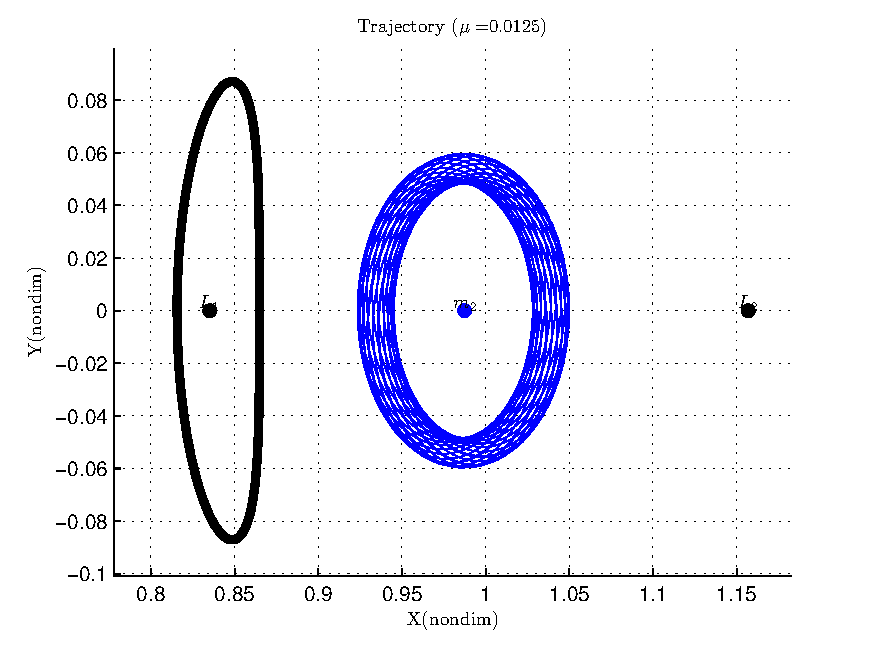
\includegraphics[width=0.7\textwidth]{2015AAS/moon_orbit.pdf}
    \end{figure}
    
    \note[itemize]{
        \item Introduce problem
        \item Possible use as a communication array
        \item Might actually be a distant retrograde orbit
        }
\end{frame} %--------------------------------------------%

\begin{frame}%------------------------------------------------%
\frametitle{Reachable Set Transfer}
\begin{itemize}
    \item Reachablility set generated on Poincar\'e section
    \item<3-> Intersection point used to generate a transfer
\end{itemize}
    \begin{figure} 
    \centering 
    \begin{subfigure}[htbp]{0.5\textwidth} 
        \only<1-2>{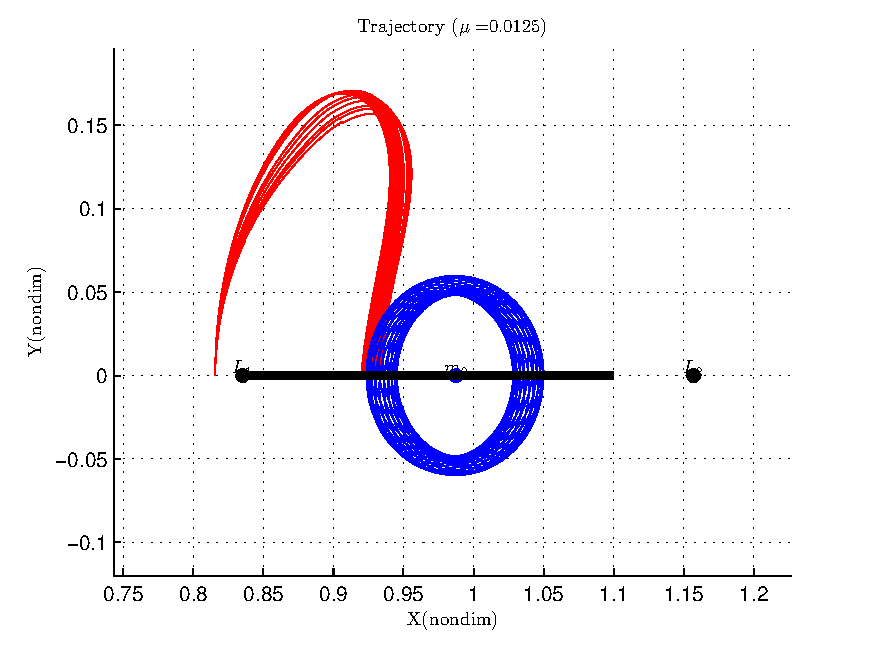
\includegraphics[width=\textwidth]{2015AAS/reach_trajectory}  }
        \visible<3->{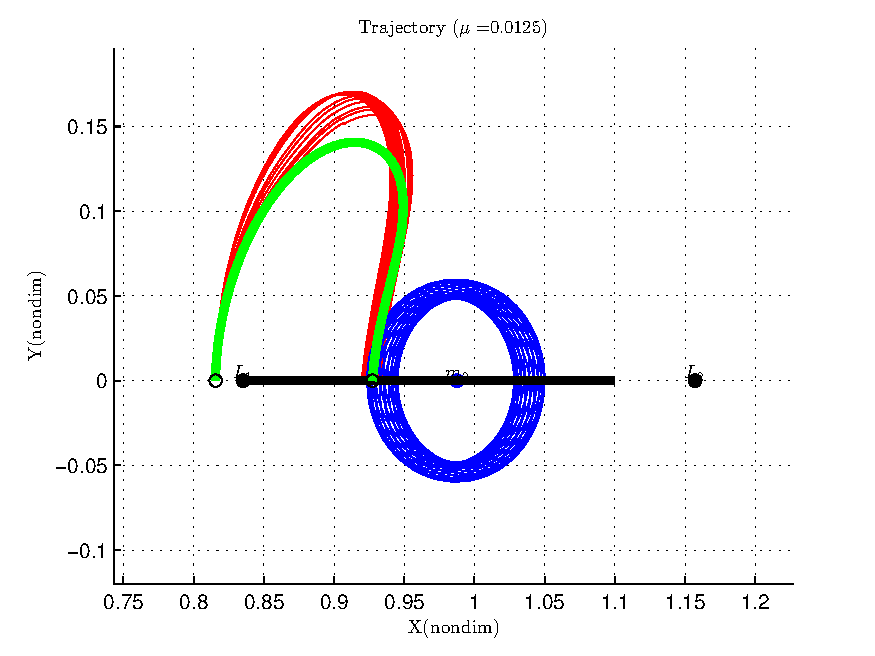
\includegraphics[width=\textwidth]{2015AAS/reach_transfer}  }
    \end{subfigure}~
    \begin{subfigure}[htbp]{0.5\textwidth} 
        \visible<2->{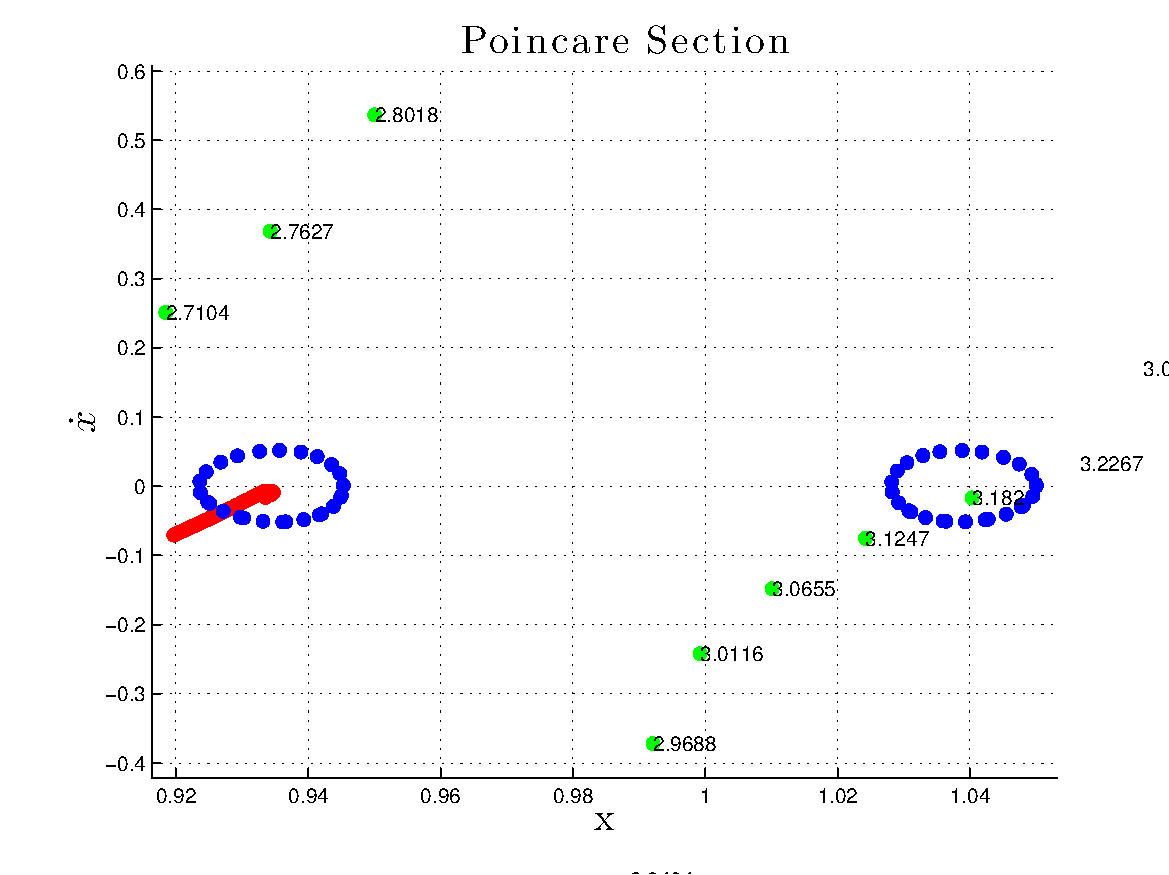
\includegraphics[width=\textwidth]{2015AAS/poincare_compare} }
    \end{subfigure} 
    \end{figure}
    
        \visible<4->{
    \begin{itemize}
        \item  Reachable set intersect the target 
        \item Shorter time of flight \( t_f \approx 1.4 \)
    \end{itemize}
    }
    \note[itemize]{
        \item Compare to reachable set approach
        \item Shorter time of flight
        \item Multiple shooting to solve TPBVP
        Vary \( \theta\) to change direction on section
        Linear interpolation to determine intersection on Poincar\'e section
        }
\end{frame} %--------------------------------------------------%

% Differences when considering an asteroid - polyhedron model

\begin{frame}{Polyhedron Gravitation Model}

\begin{itemize}
    \item Potential is a function of only the shape model
    \item Globally valid, closed-form expression of potential
    \item Exact potential assumes a constant density 
    \item Accuracy solely dependent on shape model
\end{itemize}
\only<2>{
\begin{align*}\label{eq:potential}
    U(\vecbf{r}) &= \frac{1}{2} G \sigma \sum_{e \in \text{edges}} \vecbf{r}_e \cdot \vecbf{E}_e \cdot \vecbf{r}_e \cdot L_e - \frac{1}{2}G \sigma \sum_{f \in \text{faces}} \vecbf{r}_f \cdot \vecbf{F}_f \cdot \vecbf{r}_f \cdot \omega_f 
\end{align*}
}
\only<3>{
\begin{center}
  \animategraphics[autoplay,loop,width=0.5\textwidth]{30}{./animation/castalia/IMG}{00001}{00999}~\hfill
  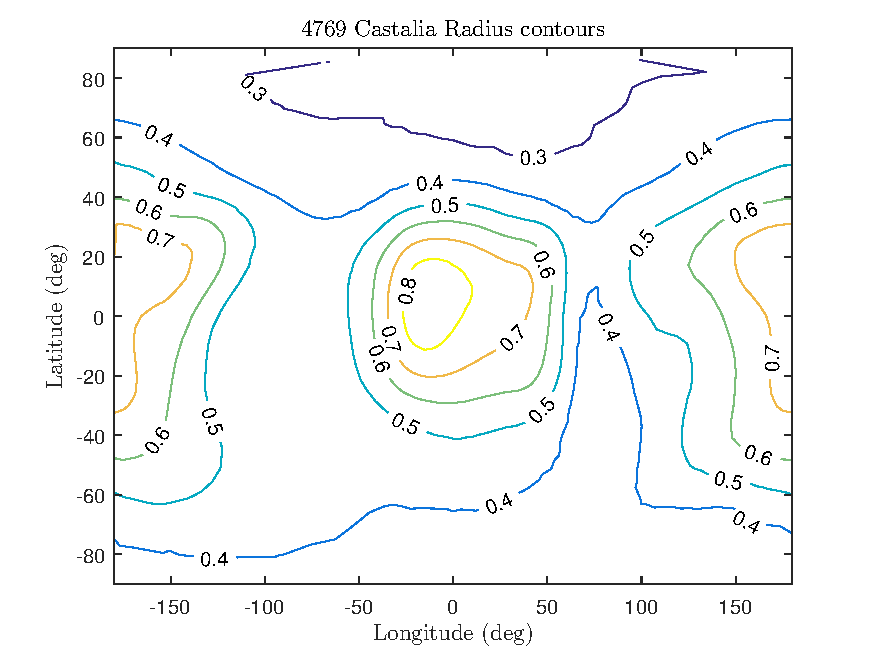
\includegraphics[width=0.5\textwidth]{figures/radius_contour.pdf}
\end{center}
}

\end{frame}

\subsection*{Asteroid transfers}

\begin{frame}[t]\frametitle{Asteroid Paper}
    
Extended reachability and \Poincare to more challenging enviornment 

Gravity model is much more complex and dynamics are highly perturbed

\end{frame}

% Results from 2016 AAS
\begin{frame}{Transfer Objective} %-----------------------------%

\begin{itemize}
    \item Goal is to transfer between two equatorial periodic orbits
    \item Typical scenario during study of an asteroid
\end{itemize}

\begin{center}
    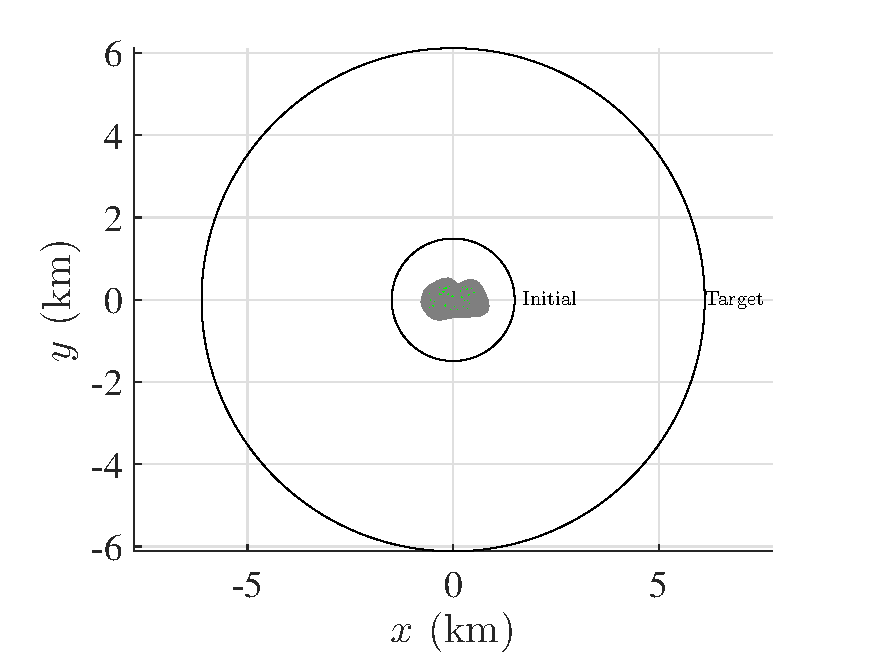
\includegraphics[width=0.5\textwidth]{figures/initial_transfer.pdf}
    \hfill
    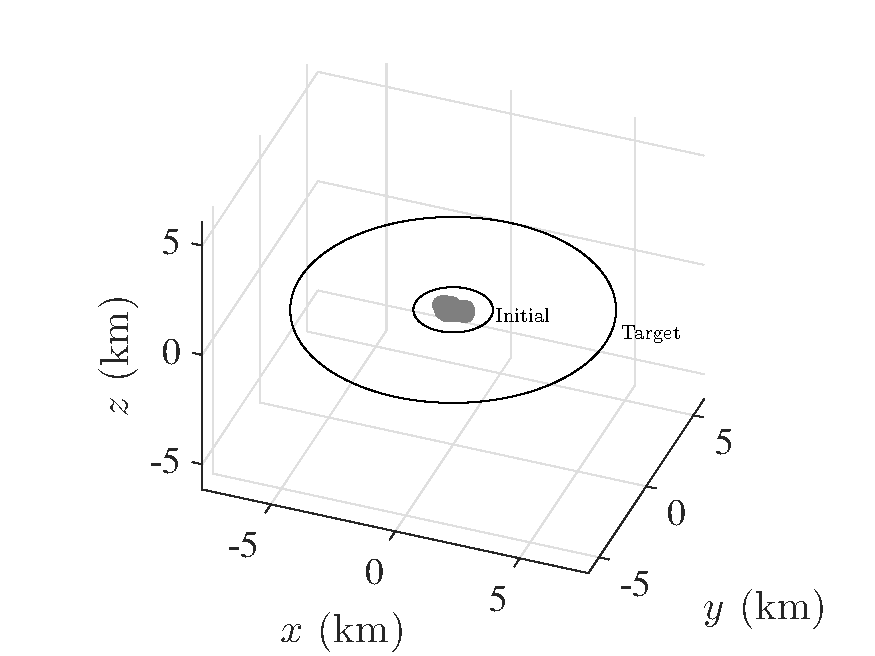
\includegraphics[width=0.5\textwidth]{figures/initial_transfer_3d.pdf}
\end{center}

\end{frame}%-----------------------------%

\begin{frame}{Simulation}


\begin{itemize}
    \item Generate the reachability set through discretization of \( \phi_i \)
    \item Visualize \( \Sigma \in \R^4 \) through the use of two 2-D sections
    \pause
    \item Control input allows for large deviation in velocity components
\end{itemize}

\begin{center}
    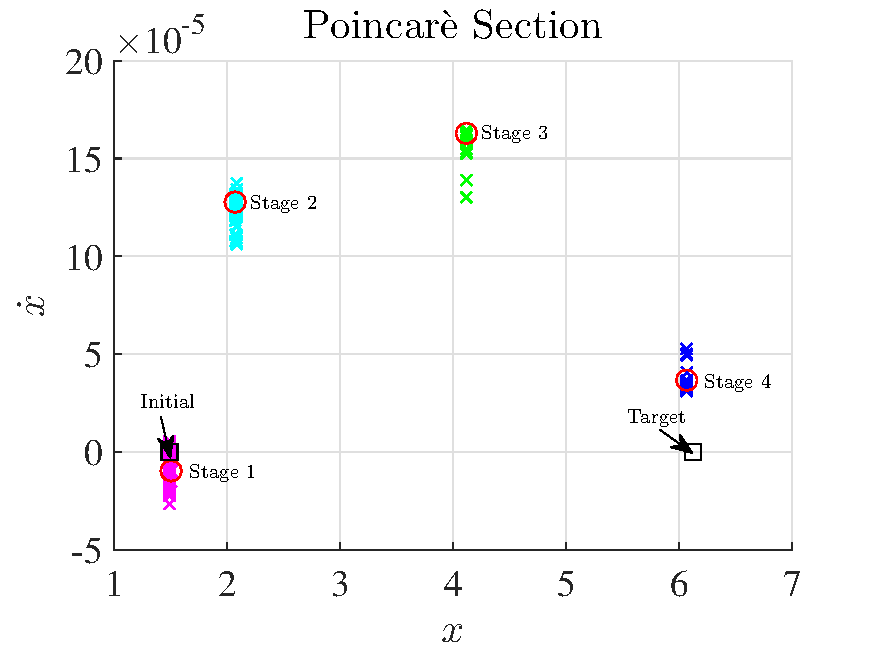
\includegraphics[width=0.5\textwidth]{figures/poincare_xvsxdot.pdf}
    \hfill
    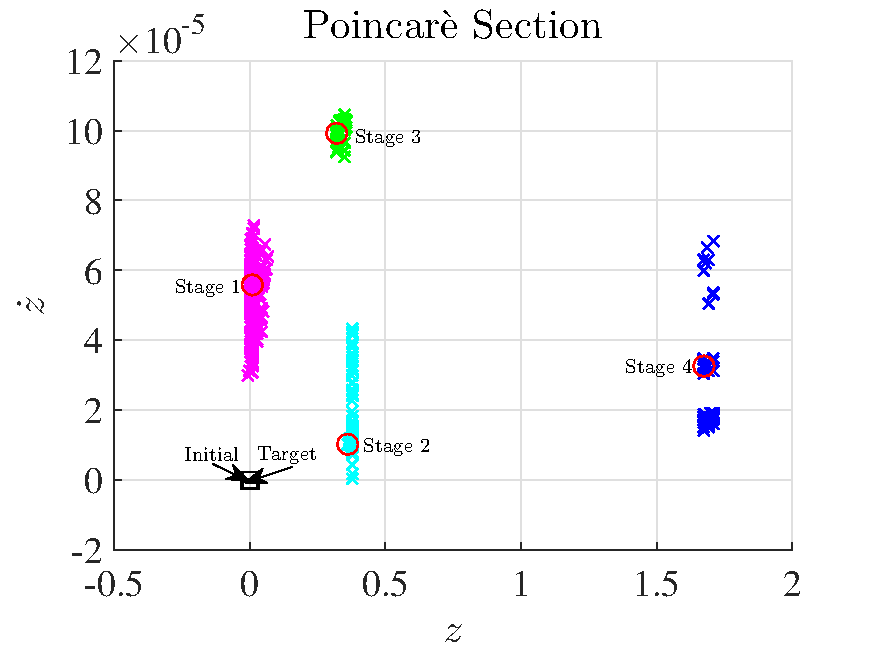
\includegraphics[width=0.5\textwidth]{figures/poincare_zvszdot.pdf}
\end{center}

\end{frame}

\begin{frame}{Simulation}
    \begin{itemize}
        \item Four iterations of the reachable state to meet the target set
        \item Final transfer is computed with a fixed terminal state constraint
    \end{itemize}

    \begin{center}
        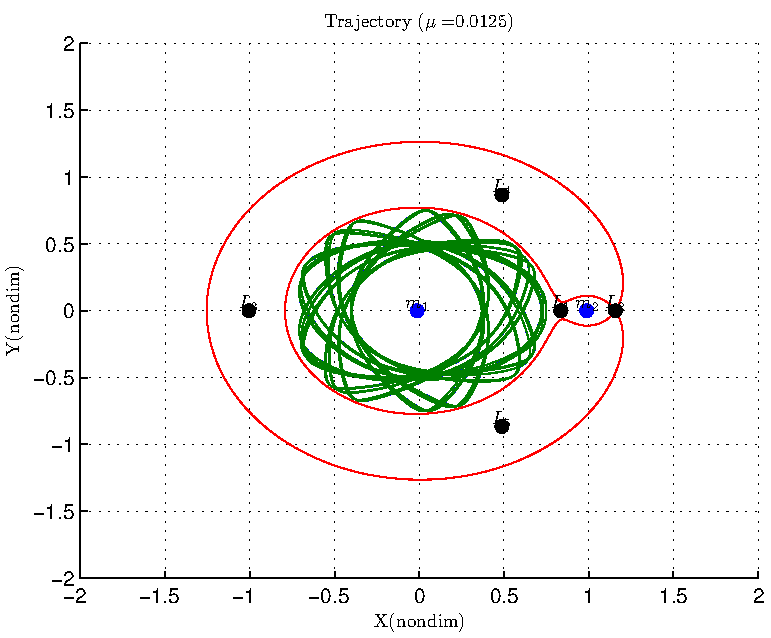
\includegraphics[width=0.5\textwidth]{figures/trajectory.pdf}
        \hfill
        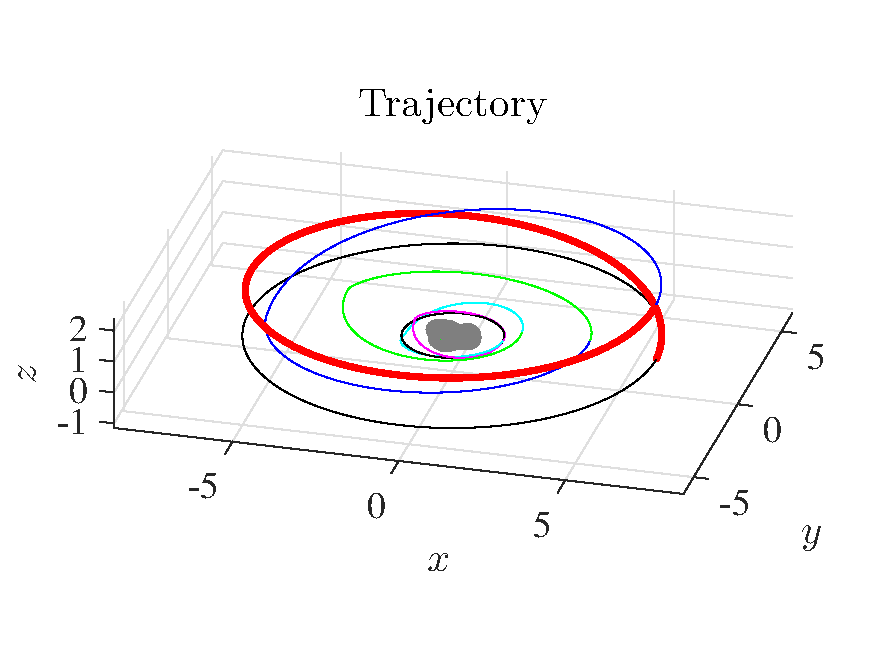
\includegraphics[width=0.5\textwidth]{figures/trajectory_3d.pdf}
    \end{center}

\end{frame}

\begin{frame}{Complete transfer}
\begin{itemize}
    \item We can visualize the complete trajectory in both the body and inertial frames
\end{itemize}

\begin{center}
  \animategraphics[autoplay,loop,width=0.5\textwidth]{30}{./animation/body/IMG}{00001}{01499}~\hfill
  \animategraphics[autoplay,loop,width=0.5\textwidth]{30}{./animation/inertial/IMG}{00001}{01499}
\end{center}

\end{frame}

\subsection*{Constrained Attitude Control}


% Results from 2016 ACC

\begin{frame}[t]\frametitle{Constrained Attitude Control}
    
geometrically exact representation of system configuration allows for global stability

Attitude control in the presence of constraints

\end{frame}

\begin{frame}{Objective} %---------------------------------------%

    \begin{block}{Nonlinear Control Design}
        Design control input \( u \) that stabilizes system from initial attitude \( R_0 \) to desired attitude \( R_d \) while avoiding obstacles
    \end{block}
    \pause
    \vs
    \begin{itemize}
        \item Avoid drawbacks of other approaches 
        \begin{itemize}
            \item \Emph{Geometric control} - analysis is conducted directly on \( \SO \) 
            \item \Emph{Barrier function} - allows for arbitrary amount of constraints
            \item \Emph{Efficient } - real time feedback control
            \item \Emph{Stability} - Lyapunov analysis gives rigourous stability proof
            \item \Emph{Adaptive} - handles system uncertainties
        \end{itemize}
    \end{itemize}
\end{frame}

\begin{frame}{Configuration Error Function} %-----------------------------%
\only<1>{
\begin{itemize}
    \item Error function quantifies ``distance'' to desired attitude
    \begin{align*}
            \Psi(R, R_d) = A(R, R_d) B(R) .
    \end{align*}
    \vs
    \item Combination of attractive and repulsive terms   
\end{itemize}
\begin{gather*}
    A(R, R_d) = \frac{1}{2} \tr{G \left( I - R_d^T R\right)} . \\ \\
    B_i(R) = 1 - \frac{1}{\alpha_i} \ln \left( - \frac{ r^T R^T v_i - \cos \theta_i}{1 + \cos \theta_i}\right) .
\end{gather*}     
}

\only<2>{
    \begin{itemize}
        \item Attractive well at the desired attitude
    \end{itemize}
    \begin{align*}
        A(R,R_d) = \frac{1}{2} \tr{G \left( I - R_d^T R\right)} .
    \end{align*}
    \begin{figure} 
        \centering
        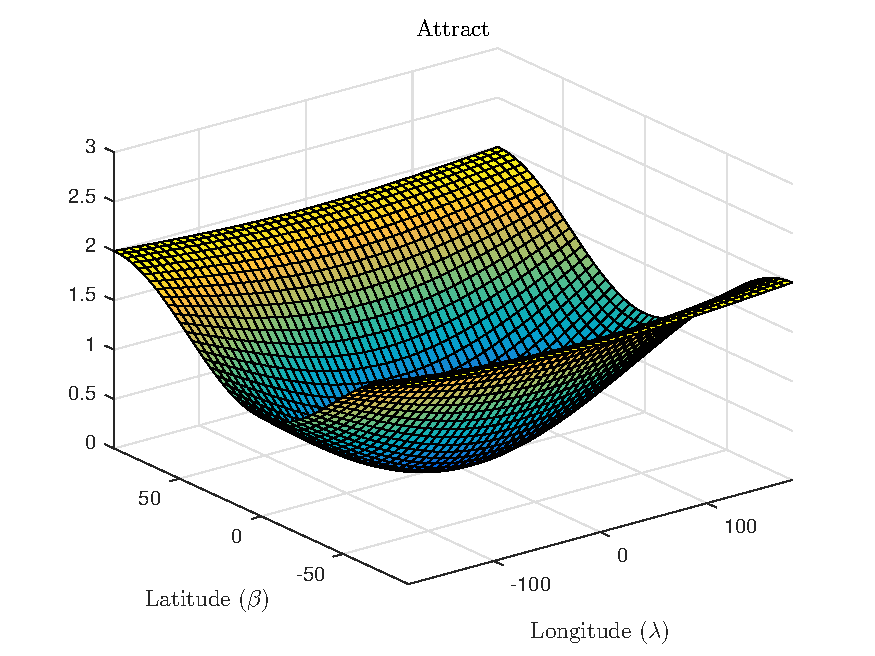
\includegraphics[height=0.6\textheight]{attract_error}
    \end{figure}
}

\only<3>{
    \begin{itemize}
        \item Define a barrier around obstacles
    \end{itemize}
    \begin{align*}
        B_i(R) = 1 - \frac{1}{\alpha_i} \ln \left( - \frac{ r^T R^T v_i - \cos \theta_i}{1 + \cos \theta_i}\right).
    \end{align*}
    \begin{figure}
        \centering
        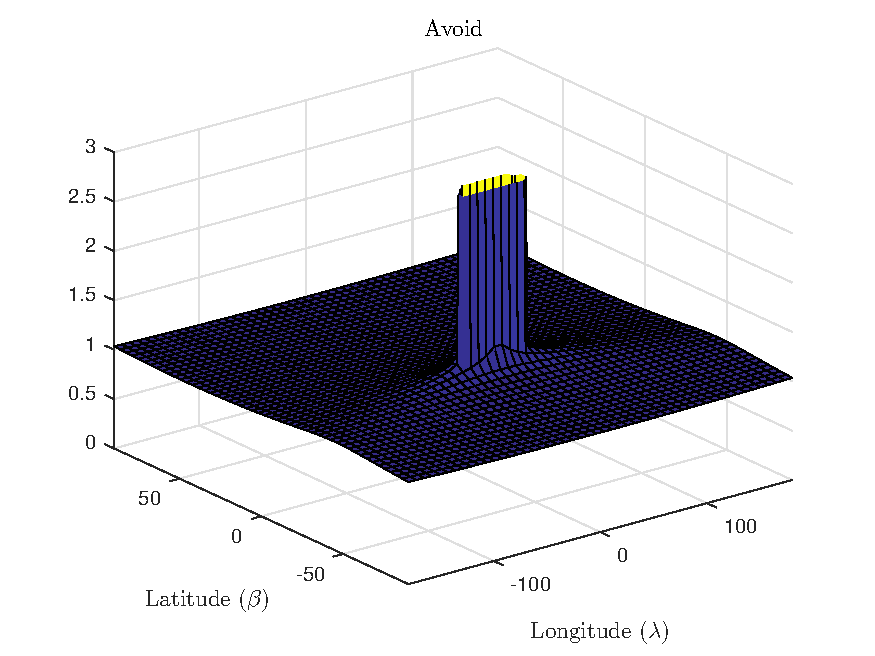
\includegraphics[height=0.6\textheight]{avoid_error}
    \end{figure}

}

\only<4>{
    \begin{itemize}
        \item Configuration error: \( \Psi : \Q \times \Q \to \R \) with control chosen to follow slope of \( \Psi \) to minimum at \( R_d\)
    \end{itemize}
    \begin{align*}
        \Psi(R, R_d) = A(R,R_d) B(R) .
    \end{align*}
    \begin{figure}
        \centering
        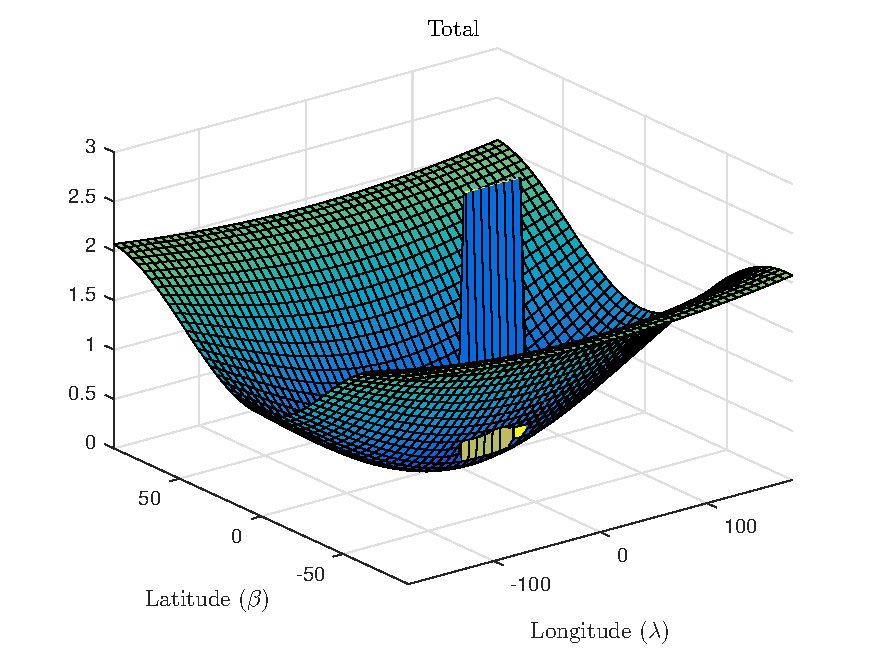
\includegraphics[height=0.6\textheight]{combined_error}
    \end{figure}
}
\end{frame}   %-----------------------------%

\begin{frame}{Numerical Simulation} %-----------------------------%

\begin{itemize}
    \item Simulate a S/C completing a yaw rotation
    \item Single obstacle in the path of sensor
\end{itemize}

\animategraphics[autoplay,loop,width=0.5\textwidth]{8}{./animation/single_noavoid/single_noavoid-}{0}{99}~
\animategraphics[autoplay,loop,width=0.5\textwidth]{8}{./animation/single_avoid/single_avoid-}{0}{99}

\end{frame}%-----------------------------%

\begin{frame}{Multiple obstacles}%-------------------------------------%

\begin{itemize}
    \item Easily handle multiple arbitrary constraints 
    \begin{align*}
        \Psi = A(R) \bracket{1 + \sum_i C_i(R)} \quad C_i = B(R) - 1
    \end{align*}
\end{itemize}

\begin{figure}
    \centering
    \animategraphics[autoplay,loop,width=0.5\textwidth]{8}{./animation/multiple_avoid/multiple_avoid-}{0}{99}
\end{figure}

\end{frame}%---------------------------------------%

\subsection*{Hardware Implementation}

\begin{frame}{Hexrotor Experiment} %-----------------------------%
\begin{itemize}
    \item Attached to spherical joint to allow only attitude dynamics
\end{itemize}
\begin{figure}
\centering
\movie[externalviewer,height=0.7\textheight]{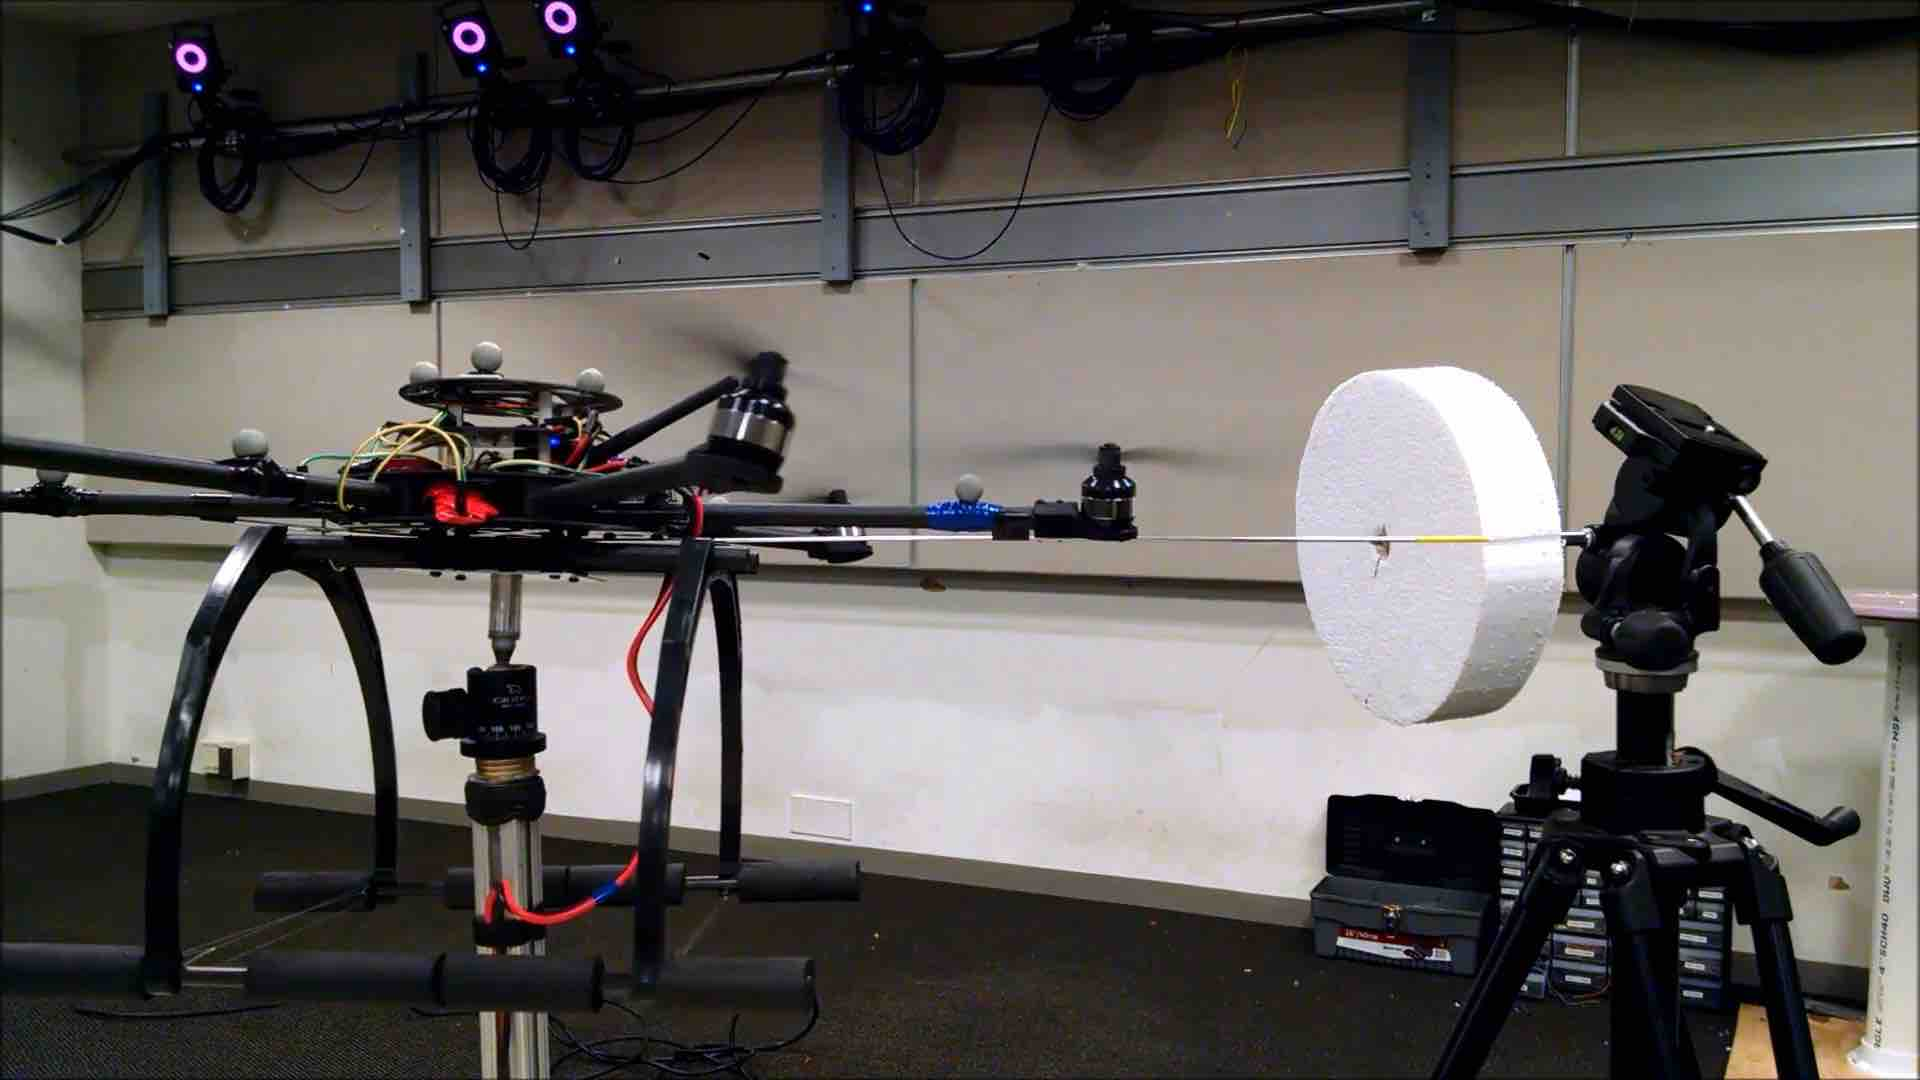
\includegraphics[height=0.7\textheight]{hexrotor}}{experiment.mp4} 
\end{figure}
\end{frame}   %-----------------------------%